\documentclass{report}
\usepackage[portuguese]{babel}
\usepackage{graphicx} % Required for inserting images

\usepackage[affil-it]{authblk} % titulo com instituição

\usepackage{listings}
\usepackage[letterpaper,top=2cm,bottom=2cm,left=3cm,right=3cm,marginparwidth=1.75cm]{geometry}
\usepackage{float}
\usepackage{makecell}
\usepackage{listings}
\usepackage[colorlinks=true, allcolors=black]{hyperref}
\usepackage{amsmath}

\usepackage{array}
\usepackage{longtable}
\usepackage{xcolor} % Pacote para adicionar cores
\usepackage{multicol}

\lstset{ % Configurações globais para listings
    basicstyle=\ttfamily, % Fonte do texto
    keywordstyle=\color{blue}, % Cor das palavras-chave
    commentstyle=\color{green}, % Cor dos comentários
    stringstyle=\color{red}, % Cor das strings
    numbers=left, % Onde os números das linhas devem ser exibidos
    numberstyle=\tiny, % Estilo dos números das linhas
    frame=single, % Adiciona uma borda ao redor do código
    %mathescape=true
}

\lstset{
    language=Makefile, 
    basicstyle=\ttfamily,
    captionpos=b,    
}


\lstdefinestyle{verilog-style}{
    language=Verilog,                    % Define a linguagem como Verilog
    basicstyle=\ttfamily\footnotesize,   % Define o estilo do texto
    keywordstyle=\color{blue},           % Cor das palavras-chave
    stringstyle=\color{red},             % Cor das strings
    commentstyle=\color{green!50!black}, % Cor dos comentários
    numbers=left,                        % Mostra a numeração de linhas à esquerda
    numberstyle=\tiny\color{gray},       % Estilo dos números de linha
    stepnumber=1,                        % Numerar cada linha
    frame=single,                        % Coloca uma borda em torno do código
    captionpos=b,                        % Coloca a legenda na parte inferior
    breaklines=true,                     % Quebra linhas longas automaticamente
    tabsize=4,                            % Define o tamanho da tabulação
    %mathescape=true
}

\lstdefinelanguage{LPF}{
    morekeywords={LOCATE, IOBUFFER, FAST, SLEWRATE, DRIVE, CLOCK, FREQUENCY},
    sensitive=false,
    captionpos=b,
}


\frontmatter  % Parte inicial sem numeração de capítulos
\title{Utilizando FPGAs com ferramentas \textit{OpenSource}}
\author{Julio Nunes Avelar %
    \thanks{Endereço de e-mail: \texttt{julio.avelar@students.ic.unicamp.br}}}
\affil{Departamento de sistemas de computação, Universidade estadual de campinas}
\date{30 de Agosto de 2024}

\begin{document}

\maketitle

\newpage
\thispagestyle{empty}  % Remove numeração da página
\vspace*{7cm}  % Espaçamento para centralizar o texto na página
\begin{flushright}
    \textit{Para minha querida paixão platônica: mesmo que você provavelmente nunca saiba disso, desde que te conheci, seu lindo sorriso e toda a sua perfeição têm me incentivado a ser uma pessoa melhor a cada dia.}  % Texto da dedicatória
\end{flushright}

\chapter*{Prefácio}
\addcontentsline{toc}{chapter}{Prefácio}

Nos últimos anos, a indústria esteve sempre dois passos à frente da academia no campo da síntese de hardware, com a maioria das ferramentas de design sendo de origem proprietária. No entanto, esse cenário começou a mudar recentemente, com o surgimento de ferramentas \textit{open-source} para o desenvolvimento de hardware e o rápido crescimento da comunidade de Hardware Livre.

Graças a essas mudanças, hoje temos a possibilidade de utilizar FPGAs (Field-Programmable Gate Arrays) e desenvolver ASICs (Application-Specific Integrated Circuits) por meio de fluxos completamente \textit{open-source}. Este manual foi escrito com o intuito de facilitar o primeiro contato com essas ferramentas, oferecendo um caminho claro para o leitor explorar esse vasto universo.

Como base, foi utilizado a toolchain \textit{open-source} OSS-CAD-Suite, que inclui o sintetizador Yosys, a ferramenta de placement and routing NextPNR, e os utilitários de geração de bitstream associados. Além disso, a principal plataforma abordada é a placa de desenvolvimento Colorlight i9, equipada com a FPGA Lattice ECP5 45f, amplamente suportada pelas ferramentas \textit{open-source}, e com o design de sua PCI disponibilizado de forma aberta.

Este manual, além de ser focado nessa plataforma, também será útil para a utilização de outras plataformas, fornecendo uma base sólida para explorar diferentes possibilidades no desenvolvimento de hardware.

Por último, gostaria de esclarecer que, embora em alguns momentos seja citado um pouco sobre design de hardware, este manual não tem como objetivo ensinar o desenvolvimento de hardware em si, mas sim como utilizar as ferramentas \textit{open-source} para esse fim. Para aprender sobre desenvolvimento de hardware, recomendo o material do professor Rodolfo Azevedo, do Instituto de Computação da Unicamp\footnote{Disponível em: \url{https://www.ic.unicamp.br/~rodolfo/Cursos/verilog}}.

Aproveito para expressar minha gratidão a todos que contribuíram para a realização deste trabalho. Em especial, agradeço ao meu orientador, Rodolfo Azevedo, por me proporcionar a oportunidade de utilizar todas as FPGAs descritas neste manual, além de seu apoio e orientação inestimáveis ao longo do processo. Também sou grato aos meus colegas de laboratório e amigos que me ajudaram com suas sugestões e feedbacks. Por fim, agradeço à minha família, que sempre esteve ao meu lado.\\

\noindent
Boa leitura e boas implementações!\\

\noindent
\textit{Julio Nunes Avelar}

\tableofcontents
\mainmatter  % Inicia o corpo principal do livro, com numeração de capítulos.
\chapter{Conhecendo o Ferramental}

\section{Introdução}

Antes de iniciarmos a utilização das ferramentas para o desenvolvimento de hardware, é essencial que conheçamos cada uma delas e tenhamos em mente o que são capazes de fazer e para que servem. Ao contrário das ferramentas proprietárias, que geralmente possuem poucos utilitários responsáveis por uma grande quantidade de funções, as ferramentas \textit{open-source} oferecem maior flexibilidade, mas também são mais fragmentadas, com o fluxo sendo composto por diversas ferramentas, cada uma responsável por uma pequena parte do processo.

Neste capítulo, exploraremos parte do conjunto de ferramentas disponível no OSS-CAD-Suite, abrangendo desde a síntese, passando pelo posicionamento e roteamento, até chegar ao carregamento na FPGA.

Falando um pouco mais sobre o OSS-CAD-Suite: trata-se de um conjunto de ferramentas para desenvolvimento de hardware, sendo que todas as ferramentas incluídas são \textit{open-source}, ou seja, não há qualquer dependência de ferramentas proprietárias.

\section{O fluxo de Design de circuitos digitais}

O fluxo de design de circuitos digitais, de maneira geral, inicia-se com a descrição do circuito a ser construído por meio de uma linguagem de descrição de hardware (Hardware Description Language - HDL), através de um nível de descrição que chamamos de RTL (Register Transfer Level), onde o circuito é descrito de forma comportamental. As linguagens mais utilizadas para essa tarefa atualmente são Verilog, SystemVerilog e VHDL.

Após a descrição do circuito, ele passa por um processo de síntese, onde é convertido para um nível de descrição chamado Gate Level. Nesse nível, o hardware é representado por uma lista de malhas ou redes (Netlist, em inglês) de portas lógicas e/ou outros elementos de maior complexidade. Antes da síntese, é realizada uma verificação formal para garantir que o hardware descrito esteja livre de bugs ou falhas de especificação. Após o processo de síntese, geralmente é realizada uma verificação de equivalência entre a Netlist gerada e o circuito descrito em nível RTL, garantindo a correção da transformação.

Os elementos de uma Netlist variam conforme os componentes físicos disponíveis na arquitetura alvo. No caso de ASICs, por exemplo, a Netlist pode conter apenas portas lógicas simples, como NAND, NOR e NOT, além de flip-flops tipo D. Já em FPGAs, a Netlist é composta por LUTs (Look-Up Tables) e outras células complexas presentes na FPGA alvo, como somadores, multiplicadores, divisores, memórias e barrel shifters.

Com uma Netlist gerada, o fluxo se divide em dois caminhos: o primeiro para FPGAs e o segundo para ASICs. Neste manual, focaremos no primeiro caminho, deixando o segundo parcialmente descrito no apêndice.

Após a geração da Netlist, é realizado o processo de posicionamento e roteamento. Nessa etapa, decide-se onde posicionar os elementos da Netlist dentro das células limitadas da FPGA. Em seguida, é realizado o roteamento, que define como os elementos posicionados serão interligados na estrutura da FPGA.

Com o posicionamento e roteamento finalizados, podemos gerar um \textit{bitstream}, que consiste em um arquivo binário contendo a configuração dos elementos internos da FPGA. De posse deste \textit{bitstream}, podemos carregá-lo na FPGA, que, a partir desse momento, começará a se comportar conforme o circuito que descrevemos. O diagrama de todo esse processo pode ser visto na Figura \ref{fig:diagrama-fluxo-hardware}.

\begin{figure}[H]
    \centering
    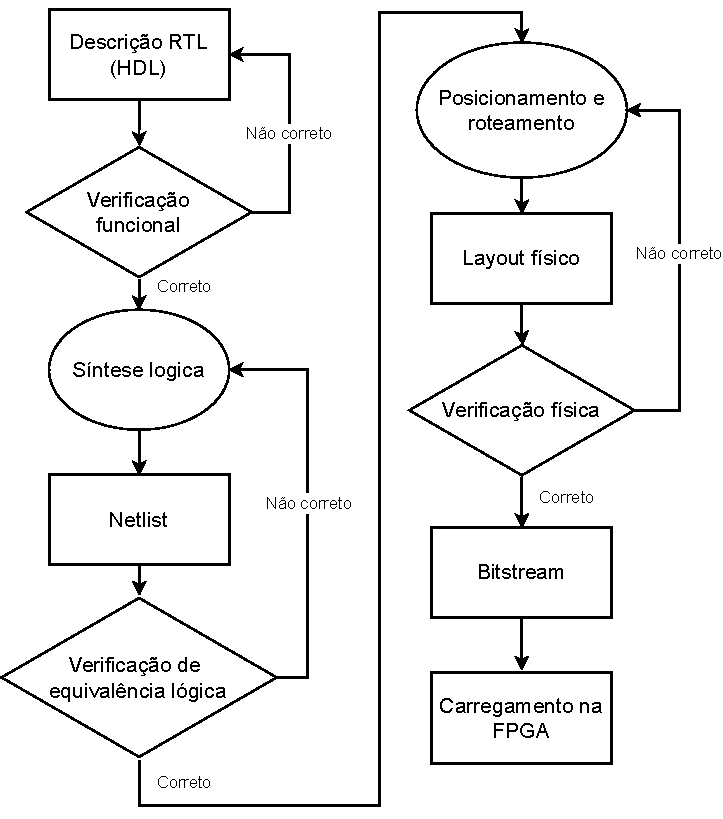
\includegraphics[width=0.9\linewidth]{hardware_levels.drawio.pdf}
    \caption{Diagrama de blocos do fluxo de design de circuitos digitais.}
    \label{fig:diagrama-fluxo-hardware}
\end{figure}

\section{As ferramentas que compõem esse fluxo}

Para a realização do fluxo descrito acima, utilizaremos quatro ferramentas distintas do OSS-CAD-Suite, cada uma responsável por uma etapa do processo.

O processo de síntese e verificação de equivalência lógica é realizado pela ferramenta Yosys (Yosys Open SYnthesis Suite) em conjunto com a ferramenta ABC (System for Sequential Logic Synthesis and Formal Verification), integrada internamente ao Yosys. O Yosys recebe como entrada um conjunto de arquivos em Verilog ou SystemVerilog. Com o auxílio de um plugin baseado no GHDL, também é possível utilizar arquivos em VHDL. A saída do Yosys é uma Netlist gerada para a arquitetura alvo, que é especificada durante o comando de síntese.

Para o posicionamento e roteamento, utilizamos o NextPnR. O NextPnR suporta diferentes FPGAs, organizadas por subprojetos dedicados a cada família de dispositivos. Assim, FPGAs de fabricantes e famílias diferentes podem ter níveis variados de suporte, dependendo do estágio de desenvolvimento do subprojeto responsável. No momento em que este manual foi escrito, o NextPnR oferece suporte às seguintes FPGAs:

\begin{enumerate}
    \item Dispositivos Lattice iCE40 - projeto IceStorm
    \item Dispositivos Lattice ECP5 - projeto Trellis
    \item Dispositivos Lattice Nexus - projeto Oxide
    \item Dispositivos Gowin LittleBee - projeto Apicula
    \item Dispositivos Altera Cyclone V - projeto Mistral
    \item Dispositivos Lattice MachXO2 - projeto Trellis
\end{enumerate}

Junto aos subprojetos do NextPnR, para cada família de FPGA, estão incluídas as ferramentas responsáveis pela geração de \textit{bitstream} para essas famílias. Como este manual utiliza a placa de desenvolvimento Colorlight i9, equipada com uma FPGA Lattice ECP5 45f, utilizaremos a ferramenta \texttt{ecppack}, incluída no projeto Trellis.

Por fim, para o carregamento do \textit{bitstream} na FPGA, utilizaremos o utilitário OpenFPGALoader, que suporta uma vasta gama de FPGAs de diferentes fabricantes.

\section{Instalação}

A instalação das ferramentas pode ser feita de várias maneiras distintas. Neste manual, descreveremos duas opções principais: 1) a instalação através do download do pacote completo do OSS-CAD-Suite, que contém todas as ferramentas; e 2) a instalação através do gerenciador de pacotes da sua distribuição Linux.

\subsection{Vantagens e Desvantagens de Cada Método}

A instalação do OSS-CAD-Suite oferece a principal vantagem da praticidade, pois inclui todo o conjunto de ferramentas em um único pacote. No entanto, essa abordagem apresenta desvantagens, como a necessidade de atualização manual das ferramentas e a utilização de versões \textit{nightly}, além de ocupar mais espaço em disco devido ao amplo conjunto de ferramentas incluídas.

Por outro lado, ao utilizar a versão do gerenciador de pacotes, podemos contar com versões estáveis e atualizações automáticas junto ao sistema, além de um menor consumo de espaço em disco. Entretanto, a desvantagem é a necessidade de instalar manualmente todos os pacotes necessários, exigindo que o usuário saiba exatamente o nome de cada um deles.

\subsection{Instalação através do OSS-CAD-Suite}

Para instalar o OSS-CAD-Suite, basta baixar o pacote disponibilizado na última \textit{release} do projeto. As \textit{releases} podem ser encontradas em: \url{https://github.com/YosysHQ/oss-cad-suite-build/releases}. Na data da redação deste manual, a última \textit{release} disponível é a de 2024-10-01. A instalação pode ser realizada da seguinte forma:

\begin{lstlisting}[language=bash]
$ cd /tmp
$ wget https://github.com/YosysHQ/oss-cad-suite-build/\
releases/download/2024-10-01/oss-cad-suite-linux-x64-20241001.tgz
$ tar xvf oss-cad-suite-linux-x64-20241001.tgz
$ mkdir -p ~/eda
$ mv oss-cad-suite ~/eda/oss-cad-suite
$ # Para usuarios de bash
$ echo "$PATH=$PATH:~/eda/oss-cad-suite/bin" >> ~/.bashrc
$ # Para usuarios de zsh
$ echo "$PATH=$PATH:~/eda/oss-cad-suite/bin" >> ~/.zshrc
\end{lstlisting}

Lembre-se de, ao realizar o download, substituir o link pelo da \textit{release} do dia.


\subsection{Instalação através do Gerenciador de Pacotes}

Para simplificar, instalaremos apenas as ferramentas necessárias para a utilização da FPGA Lattice ECP5. Além destas, também instalaremos o simulador Iverilog e a ferramenta de visualização de \textit{waveform} GTKWave.

Para usuários de ArchLinux e derivados, utilize o seguinte comando:

\begin{lstlisting}[language=bash]
$ sudo pacman -S yosys prjtrellis gtkwave iverilog openfpgaloader
$ cd /tmp
$ git clone https://aur.archlinux.org/nextpnr-ecp5-nightly.git
$ cd nextpnr-ecp5-nightly
$ makepkg -si
\end{lstlisting}

Para usuários de Debian e derivados, utilize o seguinte comando:

\begin{lstlisting}[language=bash]
$ sudo apt install openfpgaloader yosys gtkwave iverilog nextpnr-ecp5
\end{lstlisting}

Vale ressaltar que, no momento da redação deste manual, o pacote nextpnr-ecp5 está disponível apenas nas versões \textit{testing} e \textit{sid} para usuários de Debian. Para usuários de Arch, o nextpnr-ecp5 está disponível apenas na versão \textit{nightly} pelo AUR.


\chapter{A Placa Colorlight i9}

\section{Introdução}

A Colorlight i9 é uma placa de desenvolvimento \textit{open-source} participante do projeto Colorlight. Ela contém uma FPGA Lattice ECP5 45f e possui uma irmã com capacidades menores, a Colorlight i5, além de uma versão maior, a Colorlight i9 Plus. A Colorlight i5 conta com uma FPGA Lattice ECP5 25f, enquanto a i9 Plus possui uma FPGA Xilinx Arty A7 50T. As placas Colorlight i9 e i5 apresentam compatibilidade total de pinos em suas placas de expansão.

A placa de expansão possui poucos recursos integrados, delegando a funcionalidade a 10 conectores PMOD de expansão e alguns pinos de I/O fora do padrão PMOD. Além desses conectores, a placa contém um conector HDMI(somente saída de video) e alguns pinos reservados para a conexão de um módulo Ethernet.

\section{Recursos}

Além da FPGA Lattice ECP5 45f, a Colorlight i9 e sua placa de expansão incluem:

\begin{enumerate}
    \item JTAG
    \item UART
    \item SPI-Flash
    \item SDRAM
    \item 1 LED de usuário
    \item \textit{Clock} de 25MHz
    \item 2 ETH-PHY Broadcom B50612D 1Gb
\end{enumerate}

\section{Guia rápido de pinos}

O pinout da placa de extensão da Colorlight i9 pode ser visto na Figura \ref{fig:i9_v7.2_pinout}, retirada do repositório oficial do projeto Colorlight\footnote{Disponível em: \url{https://github.com/wuxx/Colorlight-FPGA-Projects}}.

\begin{figure}[H]
    \centering
    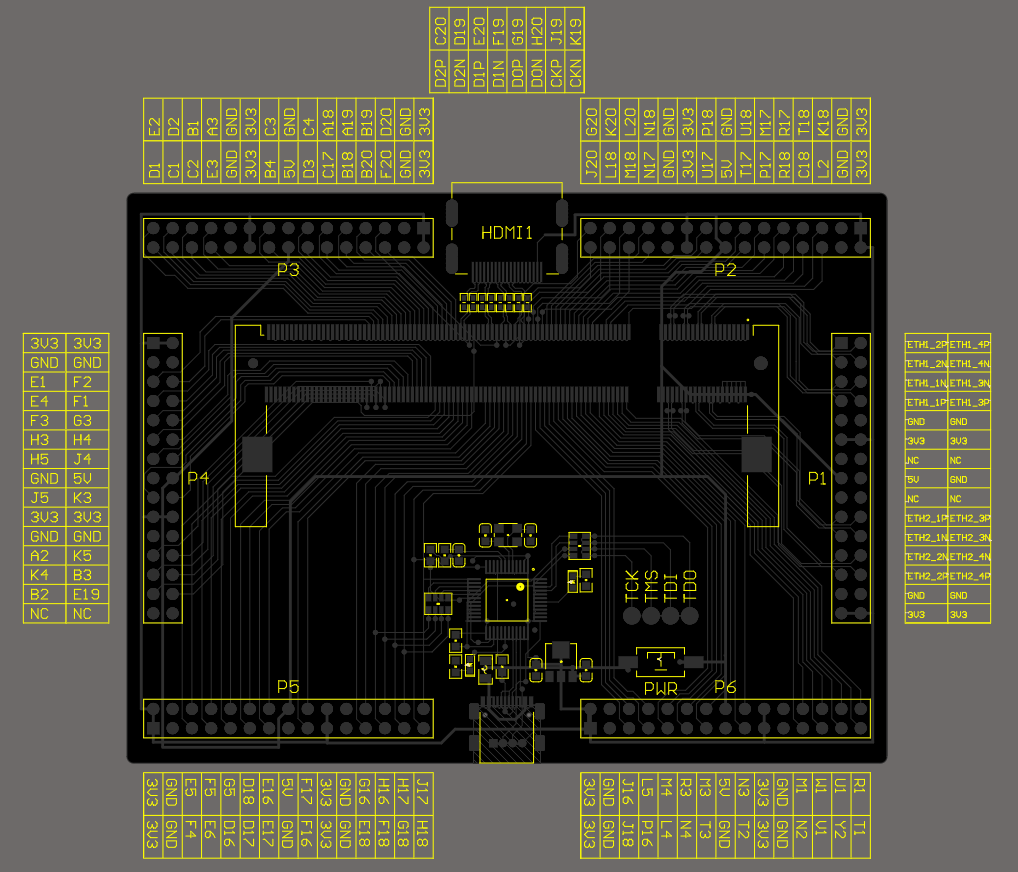
\includegraphics[width=0.75\linewidth]{i9_v7.2_pinout.png}
    \caption{Pinout da placa de extensão da Colorlight i9}
    \label{fig:i9_v7.2_pinout}
\end{figure}

Os demais pinos são apresentados a seguir:

\begin{table}[H]
\centering
\begin{minipage}{0.45\textwidth}
\centering
\begin{tabular}{|c|c|c|c|}
\hline
\textbf{Pin} & \textbf{Função} & \textbf{Pin} & \textbf{Função} \\
\hline
\multicolumn{4}{|c|}{\textbf{JTAG}} \\
\hline
J27 & TCK  & J30 & TDO \\
J31 & TMS  & J32 & TDI \\
\hline
\multicolumn{4}{|c|}{\textbf{Clock}} \\
\hline
P3 & 25 MHz clk & & \\
\hline
\multicolumn{4}{|c|}{\textbf{LED}} \\
\hline
L2 & D2 & & \\
\hline
\multicolumn{4}{|c|}{\textbf{SPI-FLASH}} \\
\hline
R2 & CS   & U3 & SCK  \\
V2 & MISO & W2 & MOSI \\
\hline
\end{tabular}
\caption{Pinout para JTAG, Clock, LED e SPI-FLASH}
\label{tab:jtag_clock_led_spi}
\end{minipage}%
\hfill
\begin{minipage}{0.45\textwidth}
\centering
\begin{tabular}{|c|c|c|c|}
\hline
\textbf{Pin} & \textbf{Função} & \textbf{Pin} & \textbf{Função} \\
\hline
\multicolumn{4}{|c|}{\textbf{SDRAM}} \\
\hline
B9  & CLK  & A11 & A9   \\
VCC & CKE  & B12 & A10  \\
GND & CS   & B6  & DQ0  \\
B10 & RAS  & A5  & DQ1  \\
A9  & CAS  & A6  & DQ2  \\
A10 & WE   & A7  & DQ3  \\
GND & DQM0 & C7  & DQ4  \\
GND & DQM1 & B8  & DQ5  \\
GND & DQM2 & B5  & DQ6  \\
GND & DQM3 & A8  & DQ7  \\
B11 & BA0  & D8  & DQ8  \\
C8  & BA   & D7  & DQ9  \\
B13 & A0   & E8  & DQ10 \\
C14 & A1   & D6  & DQ11 \\
A16 & A2   & C6  & DQ12 \\
A17 & A3   & D5  & DQ13 \\
B16 & A4   & E7  & DQ14 \\
B15 & A5   & C5  & DQ15 \\
A14 & A6   & C10 & NC   \\
A13 & A7   & C9  & NC   \\
A12 & A8   & GND & NC   \\
\hline
\end{tabular}
\caption{Pinout do SDRAM}
\label{tab:sdram}
\end{minipage}
\end{table}



A especificação de cada componente e o datasheet dos mesmos podem ser encontrados no repositório oficial do projeto Colorlight.


\chapter{Iniciando pela Teoria}

Durante o processo de desenvolvimento de hardware, uma das ferramentas mais valiosas é a simulação. Simular um design RTL e verificar o seu comportamento, seja visualmente ou formalmente, pode ser de grande utilidade ao iniciar o desenvolvimento de novos módulos de hardware ou ao procurar \textit{bugs} em um design já existente.

Para essa tarefa, o OSS-CAD-Suite fornece ferramentas de simulação como o IVerilog, Verilator e GHDL. As duas primeiras são voltadas para linguagens Verilog e SystemVerilog, enquanto o GHDL é destinado a VHDL.

Neste manual, utilizaremos o IVerilog devido à sua simplicidade e por ser perfeitamente adequado para trabalhar com Verilog sem a necessidade de outras linguagens auxiliares, como é o caso do Verilator. Apesar de suas limitações, o IVerilog é suficiente para as simulações que realizaremos.

Neste capítulo, será apresentada uma introdução ao uso do IVerilog, explicando sua sintaxe básica e como criar um \textit{testbench}, entre outros aspectos relevantes.

\section{Simulando com IVerilog}

O IVerilog utiliza arquivos de \textit{testbench} para gerar as simulações. Um \textit{testbench} nada mais é que um arquivo Verilog convencional contendo um módulo superior (\textit{top module}) e algumas diretivas específicas para simulação, como definição da unidade de tempo, geração de um sinal de \textit{clock}, ou criação de um arquivo VCD para análise dos sinais. Abaixo está um exemplo de \textit{testbench} simples:

\lstinputlisting[style=verilog-style, caption={Exemplo de Testbench - arquivo testbench\_1.v}]{testbench_1.v}

Para simularmos o \textit{testbench} acima, podemos utilizar os seguintes comandos:

\begin{lstlisting}[language=bash]
$ iverilog -o test.o -s tb_test testbench_1.v
$ vvp test.o
\end{lstlisting}

No exemplo acima, o \textit{testbench} contém um bloco always responsável por gerar o sinal de \textit{clock}, onde o registrador clk tem seu valor invertido a cada unidade de tempo. No bloco \textit{initial}, utilizamos as diretivas \$dumpfile e \$dumpvars, onde \$dumpfile especifica o nome do arquivo de saída para o \textit{waveform} e \$dumpvars define quais sinais serão "gravados" ao longo da simulação. Após um atraso de 50 unidades de tempo (definido por \#50), a simulação é finalizada com a diretiva \$finish.

Ao executar os dois comandos acima, serão gerados dois arquivos: test.o, contendo o design "compilado", e test.vcd, que armazena o \textit{waveform} com o comportamento dos sinais ao longo do tempo. O comando iverilog recebe duas \textit{flags}: -o, que define o arquivo de saída, e -s, que especifica o \textit{top module} a ser simulado.

Também é possível utilizar o IVerilog com múltiplos arquivos Verilog. Abaixo, e possível visualizar um exemplo com um módulo somador de 4 bits e seu respectivo \textit{testbench}:

\lstinputlisting[style=verilog-style, caption={Somador de 4 bits - arquivo somador.v}]{somador.v}

\lstinputlisting[style=verilog-style, caption={Testbench para o Somador - arquivo testbench\_2.v}]{testbench_2.v}

Para simular o design acima, basta rodar os seguintes comandos:

\begin{lstlisting}[language=bash]
$ iverilog -o somador.o -s tb_somador testbench_2.v somador.v
$ vvp somador.o
\end{lstlisting}

\subsection{Flags Úteis do IVerilog}

Aqui estão algumas \textit{flags} importantes para o uso do IVerilog:

\begin{enumerate}
    \item \texttt{-s}: Define o \textit{top module} da simulação.
    \item \texttt{-o}: Especifica o arquivo de saída.
    \item \texttt{-g}: Permite definir a versão da linguagem Verilog. As opções incluem: \texttt{-g1995}, \texttt{-g2001}, \texttt{-g2005}, \texttt{-g2005-sv}, \texttt{-g2009}, \texttt{-g2012}.
    \item \texttt{-D}: Permite definir macros de pré-processador para o código Verilog. Pode ser útil para passar variáveis de ambiente.
    \item \texttt{-I}: Adiciona diretórios à lista de diretórios onde o IVerilog procura por arquivos de inclusão (include).
\end{enumerate}

Essas opções podem ser combinadas conforme necessário, dependendo da complexidade do projeto. A \textit{flag} -D, por exemplo, é muito útil quando se deseja passar variáveis de ambiente diretamente na linha de comando, como demonstrado abaixo:

\begin{lstlisting}[language=bash]
$ iverilog -DDEBUG_MODE=1 -o debug.o testbench_debug.v
\end{lstlisting}

Aqui, a variável DEBUG\_MODE é definida como 1, permitindo comportamentos condicionais no código com base nessa variável.

\section{Utilizando o GTKWave}

Ao realizar uma simulação com o IVerilog, o arquivo gerado no formato VCD (\textit{Value Change Dump}) pode ser visualizado utilizando o \textit{GTKWave}, uma ferramenta de visualização de formas de onda.

Para abrir o arquivo gerado pela simulação, utilize o comando:

\begin{lstlisting}[language=bash] 
$ gtkwave test.vcd 
\end{lstlisting}

O \textit{GTKWave} permite que você inspecione os sinais do design ao longo do tempo, facilitando a depuração e compreensão do comportamento do circuito.

Principais Recursos do GTKWave:
\begin{enumerate}
    \item Zoom: Aproximação e afastamento para observar sinais em detalhes.
    \item Sinal de Interesse: Adição e remoção de sinais à janela principal para análise.
    \item Bus de Sinais: Análise de múltiplos sinais em conjunto.
    \item Anotação de Tempo: Adição de marcadores de tempo para facilitar o rastreamento de eventos na simulação.
\end{enumerate}

A Figura \ref{fig:gtkwave} mostra um exemplo de utilização do GTKWave.

\begin{figure}[H]
    \centering
    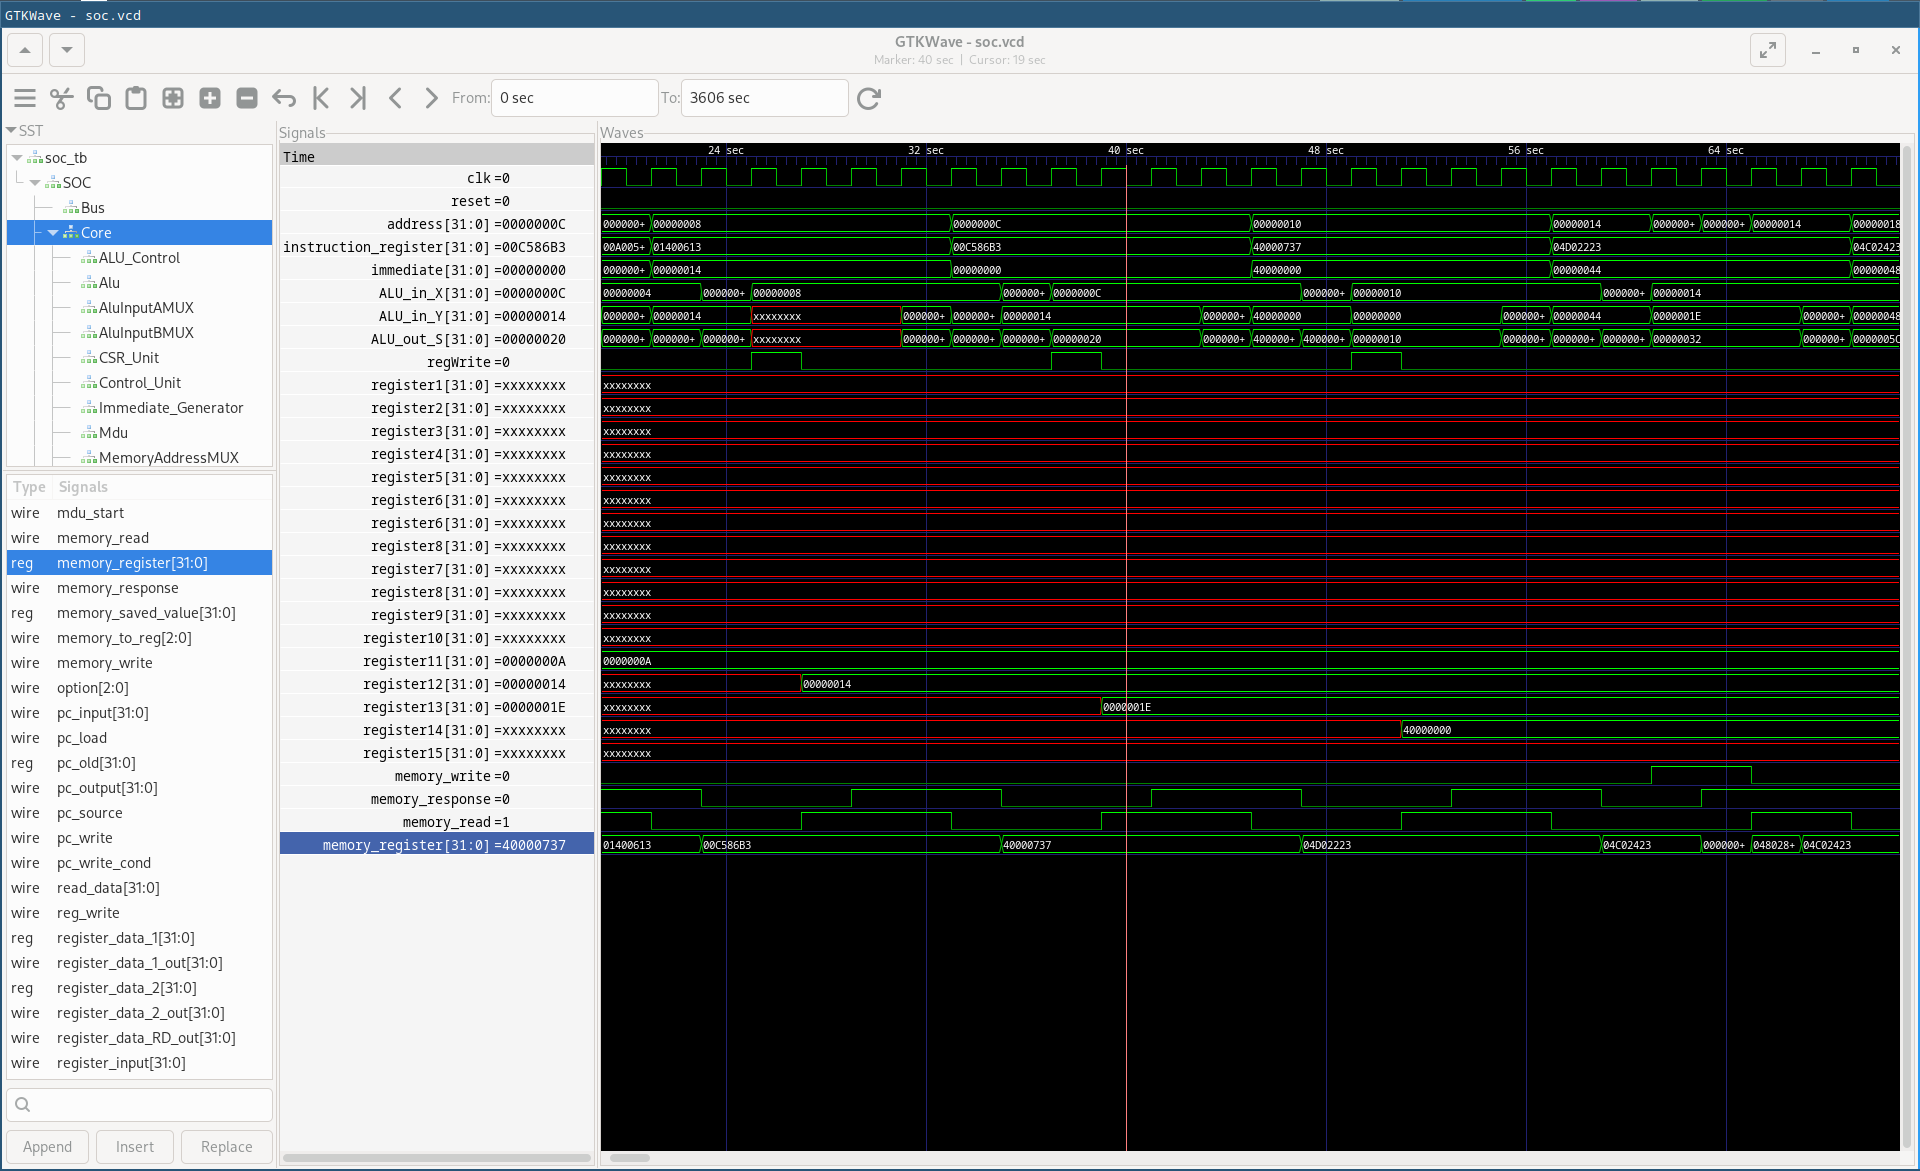
\includegraphics[width=0.8\linewidth]{gtkwave.png}
    \caption{Captura de tela do GTKWave}
    \label{fig:gtkwave}
\end{figure}

\chapter{Iniciando o Desenvolvimento}

\section{Introdução}

Até o momento, as únicas atividades realizadas foram a instalação e configuração de ferramentas, bem como a utilização de ferramentas de simulação. Neste capítulo, finalmente utilizaremos a FPGA.

\section{Definindo \textit{constraints}}

Um dos principais tipos de células disponíveis em FPGAs são as células de entrada e saída. Por meio dessas células, conseguimos fazer com que nosso design interaja com o ambiente externo, recebendo e enviando sinais.

Para utilizarmos pinos físicos da FPGA em nossos designs, precisamos informar à ferramenta de roteamento quais pinos desejamos utilizar e quais nomes daremos a eles em nosso design. Além disso, é necessário especificar informações como a tensão de operação e a frequência, caso se trate de um pino de \textit{clock}. Isso se traduz na seguinte diretriz: utilizaremos determinado pino, queremos que ele tenha um determinado alias, terá a tensão \(X\) e, se um sinal de \textit{clock} passar por ele, sua frequência será \(Y\).

Para as FPGAs da família ECP5 da Lattice, conseguimos definir essas ligações, que chamamos de \textit{constraints}, através de um arquivo LPF. Um exemplo de arquivo LPF pode ser visto abaixo:

\begin{lstlisting}[language=LPF, caption={Exemplo de arquivo .lpf}]
LOCATE COMP "clk" SITE "P3";
IOBUFFER PORT "clk" IO_TYPE=LVCMOS33;
FREQUENCY PORT "clk" 25.0 MHz;

LOCATE COMP "reset" SITE "P4";
IOBUFFER PORT "reset" IO_TYPE=LVCMOS33;

LOCATE COMP "led" SITE "L2";
IOBUFFER PORT "led" IO_TYPE=LVCMOS33;
\end{lstlisting}

Como pode ser observado no exemplo acima, definimos o nome que será atribuído a um pino físico da FPGA através da diretiva LOCATE COMP "nome a ser dado ao pino" SITE "pino físico". Em seguida, definimos o tipo do pino com IOBUFFER PORT "nome a ser dado ao pino" IO\_TYPE=tipo, e, se necessário, especificamos a frequência que passará pelo pino com FREQUENCY PORT "nome a ser dado ao pino" frequência.

\section{Um breve \textit{Blink}}

Para esclarecer a utilização das \textit{constraints} em nosso design, construiremos um exemplo onde piscamos o LED \textit{onboard} da placa, localizado no pino L2.

\begin{lstlisting}[language=LPF, caption={Arquivo blink.lpf}]
LOCATE COMP "clk" SITE "P3";
IOBUFFER PORT "clk" IO_TYPE=LVCMOS33;
FREQUENCY PORT "clk" 25.0 MHz;

LOCATE COMP "led" SITE "L2";
IOBUFFER PORT "led" IO_TYPE=LVCMOS33;
\end{lstlisting}

\begin{lstlisting}[style=verilog-style, caption={Arquivo blink.v}]
module top (
    input wire clk,
    output reg led
);

reg [31:0] counter;

initial begin
    counter = 32'h0;
    led = 1'b0;
end

always @(posedge clk) begin
    if (counter < 32'd12500000) begin
        counter <= counter + 1'b1;
    end else begin
        counter <= 32'h0;
        led <= ~led;
    end 
end

endmodule
\end{lstlisting}

Como podemos ver no exemplo acima, o nome dado ao pino no arquivo LPF é utilizado no design em Verilog. A definição de se o pino atuará como entrada ou saída fica a cargo do design e das limitações físicas da placa. Assim, ao utilizar um pino específico, é sempre aconselhável consultar o \textit{datasheet} e verificar se o pino não está associado a algum recurso específico ou possui alguma propriedade particular.

\section{Construindo o \textit{Blink}}

Na seção anterior, construímos um pequeno circuito que faz um LED piscar. Nesta seção, utilizaremos as ferramentas \textit{open-source} para sintetizar este circuito e carregá-lo na FPGA.

Para realizar a síntese do circuito, utilizaremos o seguinte comando:

\begin{lstlisting}[language=bash]
$ yosys -p "read_verilog blink.v; synth_ecp5 -json out.json -abc9"
\end{lstlisting}

Ao invocarmos o Yosys com a flag -p, estamos solicitando a execução dos comandos passados como parâmetros. Poderíamos realizar essa ação invocando o Yosys sem utilizar a flag -p, digitando comando por comando através de um \textit{shell} disponibilizado pelo Yosys, ou através de um \textit{script} TCL, utilizando a flag -c e passando o caminho para o script como parâmetro. Observando os comandos passados ao Yosys, temos um comando read\_verilog e um comando synth\_ecp5. O comando read\_verilog é responsável por ler um arquivo Verilog; assim, poderíamos utilizá-lo várias vezes para ler múltiplos arquivos Verilog. O synth\_ecp5 é responsável por iniciar a síntese. Ao passarmos a \textit{flag} -json out.json, estamos informando que queremos que a \textit{netlist} resultante da síntese seja salva no arquivo out.json. Por fim, a \textit{flag} -abc9 solicita que a versão mais recente do ABC seja utilizada. Caso não utilizemos essa \textit{flag}, apenas a versão mais antiga será utilizada. A versão mais recente do ABC é mais eficiente na simplificação da \textit{netlist}, mas, ao mesmo tempo, pode ser mais custosa e demorada em termos de tempo de síntese.

Após gerar a \textit{netlist} com o Yosys, utilizaremos o Nextpnr para realizar o posicionamento e roteamento. Para isso, utilizaremos o comando abaixo:

\begin{lstlisting}[language=bash]
$ nextpnr-ecp5 --json out.json --lpf blink.lpf --textcfg out.config \
    --package CABGA381 --45k --speed 6
\end{lstlisting}

Ao invocar o Nextpnr-ECP5 acima, fornecemos como entrada a \textit{netlist} contida no arquivo out.json, gerada pelo Yosys. Temos como saída um arquivo out.config, que contém a configuração da FPGA. Além disso, utilizamos a \textit{flag} --package para definir o encapsulamento da FPGA. No caso da Colorlight i9, esse encapsulamento é o CABGA381. Passamos a \textit{flag} --45k para definir a arquitetura da FPGA; caso fosse a Colorlight i5, por exemplo, seria --25k. Passamos também o arquivo com as \textit{constraints} com a \textit{flag} --lpf e o limite de frequência do FPGA com --speed 6. Essa constante é interna ao NextPnR e seu valor está relacionado ao modelo da FPGA; para a FPGA utilizada na Colorlight i9, o valor padrão é 6.

Com o arquivo de configuração pronto, podemos gerar nosso \textit{bitstream} utilizando o Ecppack.

\begin{lstlisting}[language=bash]
$ ecppack --input out.config --bit out.bit
\end{lstlisting}

Como opcional podemos passar ao ecppack a \textit{flag} --compress, está \textit{flag} realiza a compreensão do \textit{bitstream} e diminui drasticamente o tempo de carregamento do mesmo na FPGA.

Com o \textit{bitstream} em mãos, basta carregá-lo na FPGA com o OpenFPGALoader, utilizando:

\begin{lstlisting}[language=bash]
$ openFPGALoader -b colorlight-i9 out.bit
\end{lstlisting}

Após todo esse processo, se tudo ocorreu bem, o LED da FPGA estará piscando.

\subsection{Automatizando o Processo}

O processo de síntese descrito anteriormente é realizado completamente por linha de comando. Por esse motivo, pode ser automatizado com a utilização de um Makefile. O exemplo abaixo ilustra um Makefile que permite essa automação:

\begin{lstlisting}[language=Makefile, caption={Makefile para automatização do processo de síntese.}]
all: out.bit

out.bit: out.config
    ecppack --compress --input out.config --bit out.bit

out.config: out.json blink.lpf
    nextpnr-ecp5 --json out.json --lpf blink.lpf --textcfg out.config \
    --package CABGA381 --45k --speed 6

out.json: blink.v
    yosys -p "read_verilog blink.v; synth_ecp5 -json out.json -abc9"

load:
    openFPGALoader -b colorlight-i9 out.bit
\end{lstlisting}

Com o Makefile acima, é possível realizar todo o processo de síntese, posicionamento, roteamento e geração do \textit{bitstream} com um simples comando no terminal. Ao digitar \texttt{make}, você iniciará automaticamente todas as etapas necessárias até a geração do arquivo \texttt{out.bit}. Para carregar o \textit{bitstream} na FPGA, basta utilizar o comando \texttt{make load}. Essa abordagem não só simplifica o fluxo de trabalho, mas também minimiza a possibilidade de erros, garantindo que cada etapa do processo seja executada de maneira sequencial e na ordem correta.

\section{Utilizando PLLs}

Em muitos cenários, é necessário trabalhar com uma frequência de \textit{clock} diferente da fornecida como referência pela placa de desenvolvimento. Para obter frequências de \textit{clock} ajustadas, utilizamos PLLs (\textit{Phase-Locked Loops}), que permitem multiplicar ou dividir a frequência de um \textit{clock} de entrada.

O projeto Trellis oferece uma ferramenta chamada \texttt{ecppll}, que facilita a geração de configurações de PLL. Com essa ferramenta, é possível especificar um \textit{clock} de entrada e o \textit{clock} de saída desejado, e o \texttt{ecppll} gera um arquivo Verilog com a configuração do PLL que melhor se aproxima da frequência solicitada. 

Abaixo, e mostrado um exemplo do uso da ferramenta para gerar um \textit{clock} de 50 MHz a partir de um \textit{clock} de referência de 25 MHz, com o resultado salvo no arquivo \texttt{pll\_50.v}.

\begin{lstlisting}[language=bash]
$ ecppll -i 25 --clkin_name clki --clkout0_name clko -o 50 -f pll_50.v
\end{lstlisting}

A seguir, o código Verilog gerado pelo \texttt{ecppll}:

\begin{lstlisting}[style=verilog-style, caption={Arquivo pll\_50.v}]
module pll
(
    input clki, // 25 MHz, 0 deg
    output clko, // 50 MHz, 0 deg
    output locked
);
(* FREQUENCY_PIN_CLKI="25" *)
(* FREQUENCY_PIN_CLKOP="50" *)
(* ICP_CURRENT="12" *) (* LPF_RESISTOR="8" *) (* MFG_ENABLE_FILTEROPAMP="1" *) (* MFG_GMCREF_SEL="2" *)
EHXPLLL #(
        .PLLRST_ENA("DISABLED"),
        .INTFB_WAKE("DISABLED"),
        .STDBY_ENABLE("DISABLED"),
        .DPHASE_SOURCE("DISABLED"),
        .OUTDIVIDER_MUXA("DIVA"),
        .OUTDIVIDER_MUXB("DIVB"),
        .OUTDIVIDER_MUXC("DIVC"),
        .OUTDIVIDER_MUXD("DIVD"),
        .CLKI_DIV(1),
        .CLKOP_ENABLE("ENABLED"),
        .CLKOP_DIV(12),
        .CLKOP_CPHASE(5),
        .CLKOP_FPHASE(0),
        .FEEDBK_PATH("CLKOP"),
        .CLKFB_DIV(2)
    ) pll_i (
        .RST(1'b0),
        .STDBY(1'b0),
        .CLKI(clki),
        .CLKOP(clko),
        .CLKFB(clko),
        .LOCK(locked)
    );
endmodule
\end{lstlisting}

O \texttt{ecppll} suporta a configuração de até quatro \textit{clocks} de saída. A ferramenta oferece diversos parâmetros, sendo os principais:

\begin{itemize}
    \item \texttt{-i}: define a frequência do \textit{clock} de entrada.
    \item \texttt{--clkin\_name}: define o nome do sinal de entrada.
    \item \texttt{-o}: define a frequência do \textit{clock} de saída 0.
    \item \texttt{--clkountN}: define a frequência do \textit{clock} de saída N, onde \texttt{N} é o número da saída (0 a 3).
    \item \texttt{--clkout0\_name}: define o nome do \textit{clock} de saída 0. Para configurar saídas adicionais (até 3), use \texttt{clkoutN\_name}, onde \texttt{N} é o número da saída (0 a 3).
    \item \texttt{-f}: especifica o arquivo de saída.
    \item \texttt{--highres}: aumenta a precisão da frequência gerada.
\end{itemize}

\section{Funcionalidades Úteis do Yosys e do NextPnR}

Além das funcionalidades abordadas nos exemplos anteriores, tanto o Yosys quanto o NextPnR oferecem uma série de outras opções que podem ser extremamente úteis no desenvolvimento de projetos. Nas subseções a seguir, está  destacado algumas \textit{flags} e comandos adicionais que permitem maior controle e flexibilidade durante o processo de síntese e implementação de circuitos.

\subsection{Flags Adicionais e Comandos Úteis do Yosys}

\begin{itemize}
\item \texttt{-noabc}: O Yosys normalmente usa o otimizador ABC para simplificar a lógica combinacional. No entanto, em alguns casos, pode ser útil desativar essa etapa. A flag \texttt{-noabc} pode ser utilizada para evitar a execução do ABC.

\begin{lstlisting}[language=bash]
$ yosys -p "read_verilog mydesign.v; synth_ecp5 \
    -json out.json -noabc"
\end{lstlisting}

\item \texttt{-flatten}: O comando \texttt{flatten} no Yosys pode ser usado para converter módulos hierárquicos em um único módulo, simplificando a análise de circuitos mais complexos.

\begin{lstlisting}[language=bash]
$ yosys -p "read_verilog top.v; hierarchy -check; flatten; \
    synth_ecp5 -json out.json"
\end{lstlisting}

\item \texttt{write\_json} e \texttt{write\_verilog}: Após a síntese, é possível exportar o circuito sintetizado em diferentes formatos. O comando \texttt{write\_json} gera uma \textit{netlist} em formato JSON, enquanto \texttt{write\_verilog} escreve uma versão sintetizada do Verilog.

\begin{lstlisting}[language=bash]
$ yosys -p "synth_ecp5; write_json netlist.json"
\end{lstlisting}

\item \texttt{-D<macro>}: O Yosys permite passar macros definidos na linha de comando usando a \textit{flag} \texttt{-D}. Isso é útil para definir parâmetros de tempo de compilação, como constantes globais ou configurações específicas do projeto, diretamente no fluxo de síntese, sem precisar alterar o código Verilog.

\begin{lstlisting}[language=bash]
$ yosys -DDEBUG=1 -p "synth_ecp5 -json out.json"
\end{lstlisting}

\item \texttt{chparam}: Para ajustar parâmetros de módulos Verilog sem modificar o código original, o comando \texttt{chparam} pode ser usado para alterar parâmetros diretamente no fluxo de síntese.

\begin{lstlisting}[language=bash]
$ yosys -p "chparam -set WIDTH 16 mymodule; \
    synth_ecp5 -json out.json"
\end{lstlisting}

\item \texttt{show}: O Yosys possui um comando visual que gera um diagrama do circuito após a síntese. O comando \texttt{show} permite a visualização da netlist em formato gráfico, ajudando a inspecionar o design sintetizado.

\begin{lstlisting}[language=bash]
$ yosys -p "synth_ecp5; show"
\end{lstlisting}
\end{itemize}

\subsection{\textit{Flags} Adicionais e Casos de Uso do NextPnR}

\begin{itemize}
\item \texttt{--timing-allow-fail}: Essa \textit{flag} é utilizada para permitir que o processo de \textit{place and route} continue, mesmo que não atinja as metas de \textit{timing}. Isso é útil em designs experimentais ou quando se deseja uma primeira visualização do resultado.

\begin{lstlisting}[language=bash]
$ nextpnr-ecp5 --json out.json --lpf constraints.lpf \
    --textcfg out.config --timing-allow-fail
\end{lstlisting}

\item \texttt{--seed}: A \textit{flag} \texttt{--seed} pode ser utilizada para fornecer uma semente ao algoritmo de roteamento, o que pode ajudar a obter diferentes resultados de roteamento em execuções subsequentes, caso o primeiro não seja satisfatório.

\begin{lstlisting}[language=bash]
$ nextpnr-ecp5 --json out.json --lpf constraints.lpf \
    --textcfg out.config --seed 42
\end{lstlisting}

\item \texttt{--placer heap}: O NextPnR suporta diferentes algoritmos de posicionamento. A \textit{flag} \texttt{--placer heap} utiliza um algoritmo baseado em \textit{heap}, que pode ser mais eficiente em certos designs.

\begin{lstlisting}[language=bash]
$ nextpnr-ecp5 --json out.json --lpf constraints.lpf \
    --textcfg out.config --placer heap
\end{lstlisting}

\item \texttt{--lpf-allow-unconstrained}: Essa \textit{flag} permite que o NextPnR continue o processo, mesmo se existirem sinais que não estão explicitamente definidos no arquivo de restrições \textit{constraints}. Isso pode ser útil em designs onde nem todos os sinais estão restritos ou quando se está desenvolvendo um protótipo.

\begin{lstlisting}[language=bash]
$ nextpnr-ecp5 --json out.json --lpf constraints.lpf \
    --textcfg out.config --lpf-allow-unconstrained
\end{lstlisting}

\item \texttt{--report}: Gera relatórios detalhados sobre o design, incluindo o uso de recursos e a análise de \textit{timing}. Isso é útil para verificar a eficiência do posicionamento e para ajustar o design para melhorias.

\begin{lstlisting}[language=bash]
$ nextpnr-ecp5 --json out.json --lpf constraints.lpf \
    --textcfg out.config --report detailed_report.txt
\end{lstlisting}

\item \texttt{--detailed-timing-report}: Essa \textit{flag} gera um relatório de \textit{timing} detalhado, que pode ajudar na análise de desempenho, revelando atrasos críticos no design.

\begin{lstlisting}[language=bash]
$ nextpnr-ecp5 --json out.json --lpf constraints.lpf \
    --textcfg out.config --detailed-timing-report
\end{lstlisting}

\item \texttt{--analysis}: Essa \textit{flag} ativa uma análise adicional no design, fornecendo mais detalhes sobre possíveis problemas de \textit{timing} ou sobre a alocação de recursos.

\begin{lstlisting}[language=bash]
$ nextpnr-ecp5 --json out.json --lpf constraints.lpf \
    --textcfg out.config --analysis
\end{lstlisting}
\end{itemize}

\chapter{Aplicações Práticas e Casos de Uso}

\section{Exemplos Interessantes}

Com a Colorlight i9 e um fluxo de trabalho completamente \textit{open-source}, podemos explorar diversas aplicações práticas que permitem a utilização efetiva dos recursos da placa. Abaixo estão alguns exemplos que podem servir como inspiração:

\begin{enumerate}
    \item Controle de brilho de um LED utilizando PWM.
    \item Reprodução de músicas via PWM: \url{https://github.com/JN513/Simple-FPGA-Music-Player-with-PWM}.
    \item Integração de um ADC externo.
    \item Implementação de um eco na UART.
    \item Criação de um dispositivo SPI-Slave: \url{https://github.com/Unicamp-Odhin/SPI-Slave}.
    \item Desenvolvimento de um dispositivo SPI-Master: \url{https://github.com/Unicamp-Odhin/SPI-Master}.
    \item Comunicação entre duas FPGAs utilizando SPI.
    \item Exibição de imagens em um monitor via HDMI.
    \item Utilizacão de um RISC-V na FPGA: \url{https://github.com/JN513/Risco-5}.
\end{enumerate}

\section{Utilizando o LiteX}

O LiteX é um framework robusto que facilita a criação e uso de cores e sistemas em chip (SoCs) em FPGAs. Ele oferece suporte a várias FPGAs e inclui uma rica biblioteca de IPs e cores \textit{open-source}.

\subsection{Instalando o LiteX}

A instalação do LiteX em um sistema Linux é um processo simples. Recomenda-se criar uma pasta dedicada chamada eda (Electronic Design Automation) para gerenciar seus projetos. Para instalar o LiteX, siga os passos abaixo, conforme indicado na documentação oficial:

\begin{lstlisting}[language=bash]
$ cd
$ mkdir -p eda/litex
$ cd eda/litex
$ python3 -m venv litex_env
$ wget https://raw.githubusercontent.com/enjoy-digital/\
litex/master/litex_setup.py
$ . litex_env/bin/activate
$ python3 ./litex_setup.py --init --install --config=standard
$ echo 'alias get_litex=". $HOME/eda/litex/litex_env/bin/activate"'\
>> ~/.bashrc
$ echo 'alias get_litex=". $HOME/eda/litex/litex_env/bin/activate"'\
>> ~/.zshrc
\end{lstlisting}

A instalação ocorre em um ambiente virtual Python, e para utilizá-lo, você deve ativar o ambiente com o comando get\_litex. O processo pode levar alguns minutos, pois o LiteX clona diversos repositórios necessários para o funcionamento do framework e das ferramentas associadas.

Para aqueles que desejam se aprofundar no LiteX, os desenvolvedores disponibilizam alguns tutoriais: \url{https://github.com/litex-hub/fpga_101}.

\subsection{Utilizando o LiteX com a Colorlight i9}

Durante a instalação do LiteX, um diretório chamado litex\_boards é criado. Este diretório contém definições para as placas FPGA suportadas pelo LiteX, além de exemplos de utilização.

Para nosso teste, utilizaremos o arquivo colorlight\_i5.py, que pode ser encontrado em: litex-boards/litex\_boards/targets. Navegue até este diretório com o seguinte comando:

\begin{lstlisting}[language=bash]
$ cd ~/eda/litex/litex-boards/litex_boards/targets
\end{lstlisting}

Uma vez no diretório, ative o ambiente do LiteX e execute o script Python colorlight\_i5.py com as opções indicadas abaixo:

\begin{lstlisting}[language=bash]
$ get_litex
$ python3 colorlight_i5.py --board i9 --revision 7.2 --build --load \
    --with-video-framebuffer
\end{lstlisting}

Se tudo ocorrer como esperado, ao conectar a FPGA a um monitor HDMI, algumas cores serão exibidas na tela.

\subsection{Linux on VexRiscV}

O LiteX também oferece uma demonstração do Linux em execução no processador RISC-V VexRiscV para FPGAs, disponível em \url{https://github.com/litex-hub/linux-on-litex-vexriscv}. Essa implementação representa uma excelente oportunidade para explorar o funcionamento do Linux em um ambiente FPGA, ampliando as possibilidades de uso da Colorlight i9. Ao testar a demonstração, você terá acesso a um shell Linux através da UART e verá uma imagem semelhante à da Figura \ref{fig:linux_on_vexriscv} na saída de vídeo da FPGA.

\begin{figure}[H]
    \centering
    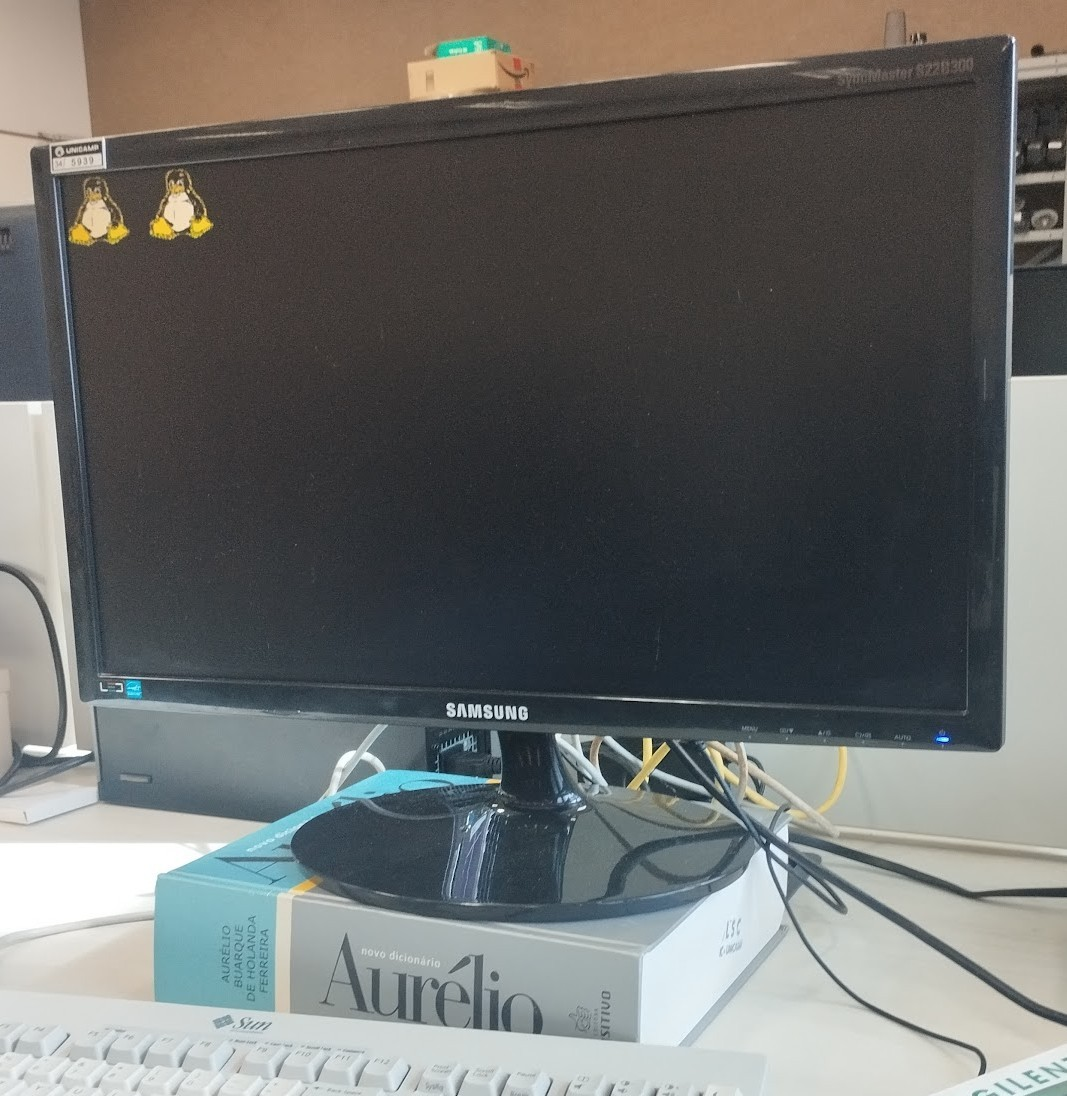
\includegraphics[width=0.5\linewidth]{linux_on_vexriscv.jpg}
    \caption{Saída de vídeo gerada pelo Linux rodando no softcore na FPGA.}
    \label{fig:linux_on_vexriscv}
\end{figure}


\chapter{Apêndice}

\section{Utilizando FPGAs Gowin}

\section{Utilizando FPGAs Xilinx}

\section{Desenvolvendo um Chip com TinyTapeout}

\end{document}
